% Chapter Template

\chapter{Ensayos y resultados} % Main chapter title
\label{Chapter4} % Change X to a consecutive number; for referencing this chapter elsewhere, use \ref{ChapterX}

En este capítulo se explican los diferentes ensayos y tareas que se realizaron para testear tanto el software desarrollado como el hardware fabricado.

%----------------------------------------------------------------------------------------
%	SECTION 1
%----------------------------------------------------------------------------------------

\section{Pruebas Realizadas}
\label{sec:pruebasHW}

Todas las pruebas realizadas se hicieron sobre el prototipo diseñado, que fue fabricado por la empresa Servaind SA. Debido a que la empresa se encuentra radicada en CABA, todas las pruebas con el prototipo fabricado fueron realizadas a distancia por medio de conexiones remotas.

\subsection{Pruebas de comunicación con el ADE7953}
En el inicio del desarrollo del software, se realizaron pruebas midiendo los pines de comunicación entre el microcontrolador y el ADE7953.

Una vez armada la comunicación dentro del programa, se midieron los tiempos de la trama de mensaje UART con un osciloscopio. También se realizaron pruebas de tiempo realizando una serie de pulsos cada milisegundo, la señal puede verse en la figura \ref{fig:Osciloscopp}.


%\begin{figure}[!htb]
%	\centering
%	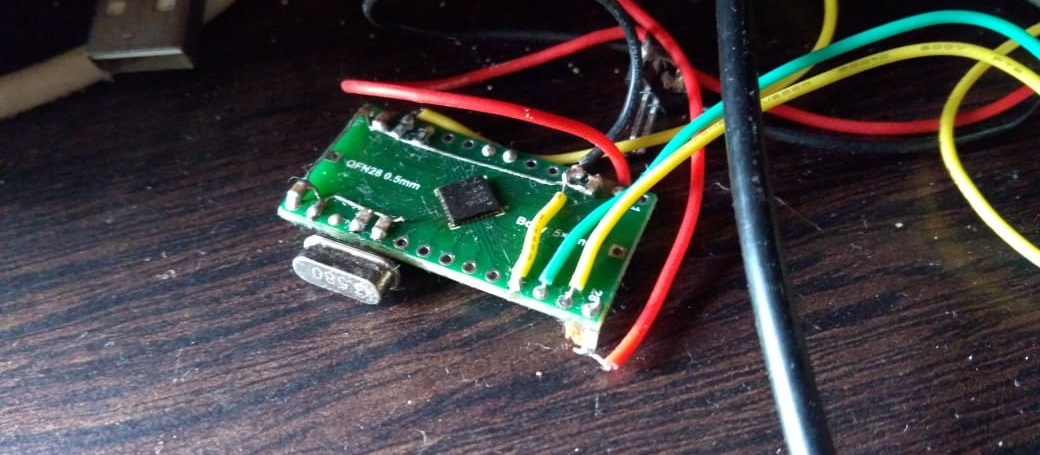
\includegraphics[width=120mm,keepaspectratio]{Figures/ADEadapt.jpg}
%	\caption{ ADE7953 soldado a adaptador.}
%	\label{fig:Adeadapt}
%\end{figure}

\begin{figure}[!htb]
	\centering
	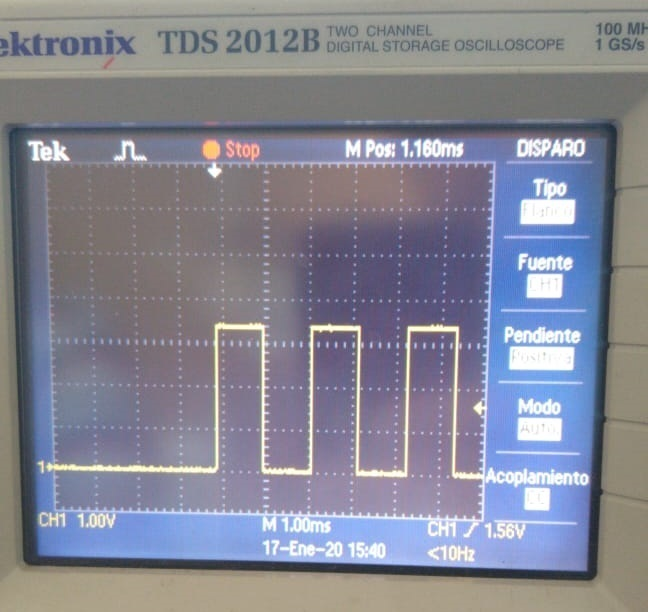
\includegraphics[width=80mm,keepaspectratio]{Figures/osciloscope.jpg}
	\caption{ Pulso de 1 milsegundo en el Osciloscopio.}
	\label{fig:Osciloscopp}
\end{figure}

En el osciloscopio se verificó que los tiempos de la trama fueran los correctos, siguiendo el esquema de la figura \ref{fig:ADEread}. Con el debugger del MSP430 se verificaron las respuestas en los registros. Se enviaron tramas para que el ADE7953 responda los registros de la tabla \ref{8biadcregis}, en la figura \ref{fig:ADEresp} se ve en la memoria del programa la respuesta al registro LAST\_ OP durante las pruebas.



\begin{figure}[!htb]
	\centering
	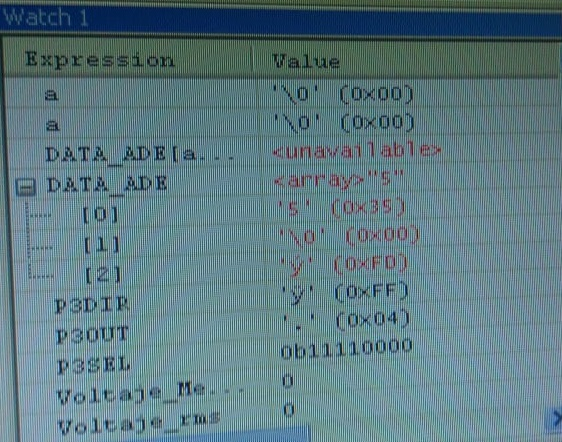
\includegraphics[width=100mm,keepaspectratio]{Figures/ADEresponse.jpg}
	\caption{ Variables leídas por el microcontrolador durante las pruebas.}
	\label{fig:ADEresp}
\end{figure}



\subsection{Testeo del protocolo Modbus}

Una vez finalizado el desarrollo del protocolo Modbus, se procedió a conectar por el puerto RS232 de la placa a la computadora del banco de trabajo. Se leyeron todos los registros disponibles. Esto puede verse en la figura \ref{fig:ModPC}. 

\begin{figure}[!htb]
	\centering
	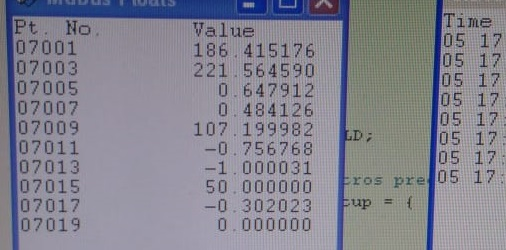
\includegraphics[width=100mm,keepaspectratio]{Figures/ModbusTest.jpg}
	\caption{ Lectura de registros Modbus en la computadora del banco de pruebas.}
	\label{fig:ModPC}
\end{figure}

Se forzaron errores para observar si el software respondía adecuadamente. Los errores probados fueron:

\begin{itemize}
\item Función ilegal
\item Dirección de dato ilegal
\item Valor de dato ilegal
\end{itemize}

Luego se testeo el mismo protocolo sobre la interfaz RS485 para asegurar que no hubiera ninguna diferencia con la interfaz RS232. Gracias a esta segunda prueba se había detectado errores en el software, la biblioteca se inicializaba cada 2 milisegundos. Al finalizar las pruebas, todos  los errores encontrados fueron corregidos.


\subsection{Testeo de la calibración}

Finalizado el desarrollo del  menú principal dentro del programa, se procedió a testear las mediciones que realizaba el dispositivo con un variador de tensión alterna y una carga conocida.
La carga conocida usada fue una lámpara de 100 W. Esta fue utilizada principalmente durante el desarrollo del programa al interpretar los valores de los registros de medición del ADE7953.
 
El variador de tensión alterna puede verse en la figura \ref{fig:BancCalib}. Este fue utilizado al finalizar el desarrollo para realizar pruebas con respecto a la calibración. Se conectó el variador al dispositivo y se probaron diferentes rangos de tensión, realizando pequeños incrementos y verificando con un multímetro. Las mediciones fueron comparadas con un multímetro digital \textquotedblleft Gw Instek Gdm360\textquotedblright.

\begin{figure}[!htb]
	\centering
	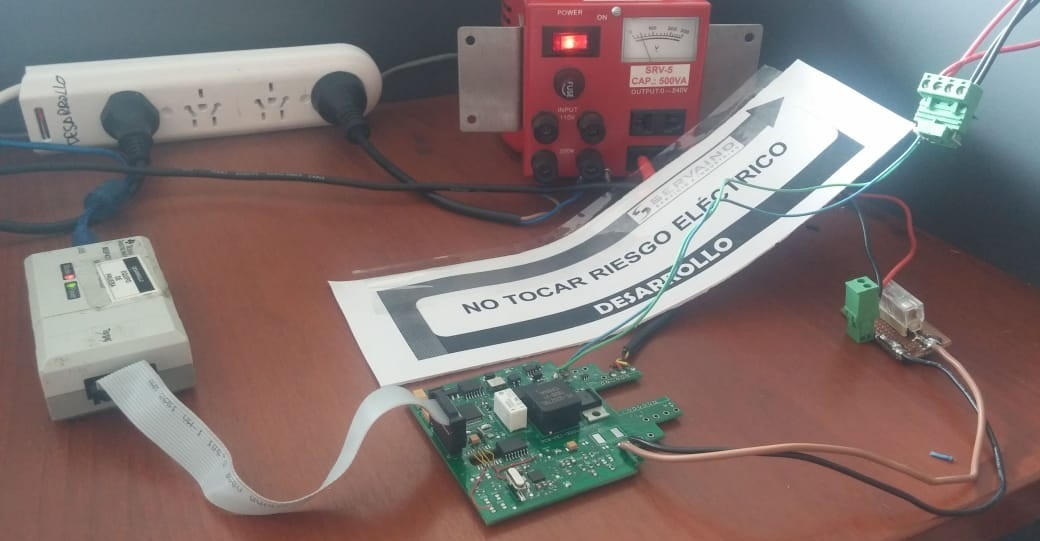
\includegraphics[width=\textwidth ,keepaspectratio]{Figures/BancoCalib.jpg}
	\caption{ Banco de pruebas con el autotransformador.}
	\label{fig:BancCalib}
\end{figure}

Los procedimientos para realizar la calibración fueron los recomendados por la hoja de aplicación del fabricante, se imitó el esquema de la figura \ref{fig:SquemCalib}.

\begin{figure}[!htb]
	\centering
	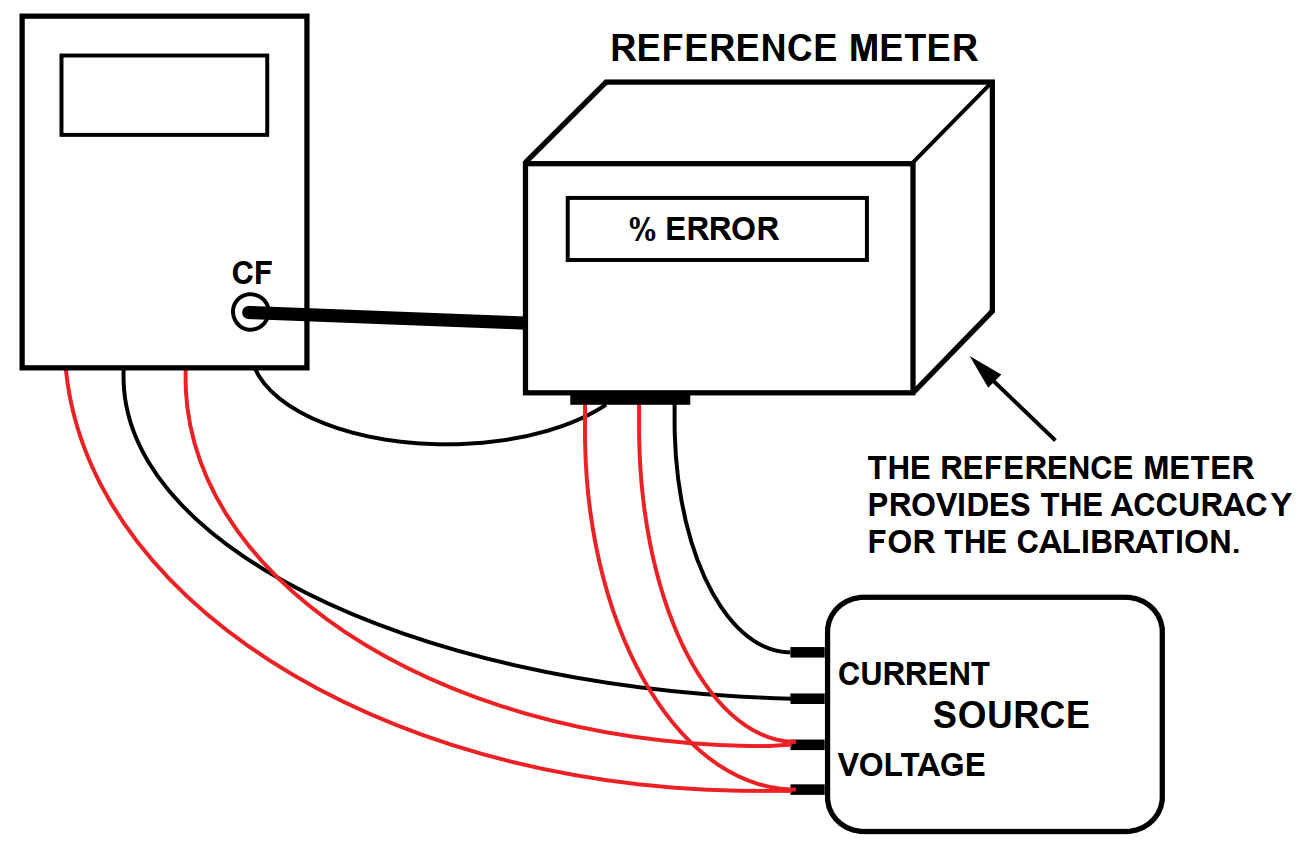
\includegraphics[width=120mm ,keepaspectratio]{Figures/HojadeAplicacion.png}
	\caption{ Esquema de calibración según la hoja de aplicación del integrado ADE7953. La hoja de aplicación denominada AN-1118, se encuentra disponible en la pagina web del fabricante\protect\footnotemark .}
	\label{fig:SquemCalib}
\end{figure}

\footnotetext{\url{https://www.analog.com/media/en/technical-documentation/application-notes/AN-1118.pdf}}

%Se utilizo el primer prototipo para hacer las pruebas. Se realizaron mediciones sobre una lampara de 100 W para probar el funcionamiento del integrado de medición y las funcionalidades del software.

%Se probo desconectar y conectar las tensiones de entrada para probar la reacción de la placa y corregir problemas que presentara en el software. Gracias a esto se detectaron errores en la comunicación 

%Se utilizaron los puertos RS232 y RS485 para probar la comunicación por protocolo modbus.

\section{ Verificación de requerimientos}

%Durante las pruebas se verificaron los requerimientos solicitados.

\subsection{Grupo de requerimientos referidos a alimentación eléctrica}
%\begin{itemize}
%\item El dispositivo deberá alimentarse con tensión continua. La tensión de alimentación deberá ser inferior a 30 V y superior a 12V.
%\end{itemize}

Se conectó el prototipo a un variador de alimentación para probar las diferentes tensiones que soporta para encenderse. Para probar su conector de alimentación, se lo conecto con un fusible. Esto puede verse en la figura \ref{fig:ConectorProoto}.



\begin{figure}[!htb]
	\centering
	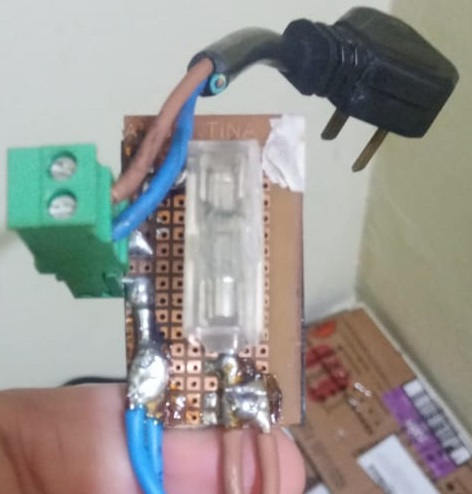
\includegraphics[width=80mm ,keepaspectratio]{Figures/ConectorAlim.jpeg}
	\caption{ Conexión del prototipo durante las pruebas.}
	\label{fig:ConectorProoto}
\end{figure}

\subsection{Grupo de requerimientos referidos a medición de potencia del equipo}

En el prototipo fabricado se implementó una resistencia shunt de 4 mili ohms para realizar mediciones hasta 10 amperes. La intensidad de corriente eléctrica que tolera el shunt de medición en el prototipo es de alrededor de 30 amperes. También se implementó un arreglo de resistores de 1 M$\Omega$
 para lograr medir efectivamente hasta 495 volts. 

Durante las pruebas,  se conectó al prototipo una carga con diferentes valores de corriente y tensión, de este modo se pudo verificar la posibilidad de medir la potencia  solicitada en los requerimientos. Las mediciones fueron comparadas con un multímetro para así lograr el objetivo de medir con tolerancias inferiores al 15\%. El valor de error se encontraba cerca del 4\%.



%\begin{itemize}
%\item Capaz de realizar la medición de tensión alterna de una línea monofásica de baja tensión de Argentina, entrada de medición para 220V o 380V con una tolerancia de +/-15\%.
%\end{itemize}

%Se logro medir tensiones alternas de una linea monofásica de baja tension con tolerancia inferior al 15\%.

%\begin{itemize}
%\item Capaz de realizar la medición de corriente alterna de una línea monofásica de baja tensión de Argentina, hasta 5 A.
%\end{itemize}

%Se implemento una resistencia shunt de 4 mili ohms para realizar mediciones hasta 10 amperes. La intensidad de corriente eléctrica que tolera el shunt es alrededor de 30 amperes.

%\begin{itemize}
%\item Capaz de realizar la medición de potencia eléctrica activa de una línea monofásica de baja tensión de Argentina, hasta 4000 W.
%\end{itemize}

%Se implemento un arreglo de resistores para lograr medir efectivamente hasta 495 volts. Por lo que se puede llegar a medir hasta la potencia solicitada.

%\begin{itemize}
%\item El sistema de medición que se utilizará para las mediciones deberá ser aislado de la salida de comunicaciones del puerto serie.
%\end{itemize}

%Todos las circuitos de medición se encuentran aislados de los puertos de comunicación serie por lo que se considera resuelto este requisito.

\subsection{Grupo de requerimientos referidos a Interfaces de comunicación}
%\begin{itemize}
%\item Deberá realizar las comunicaciones a través de protocolos RS485 y RS232.
%\end{itemize}

La interfaz RS232 fue conectada exitosamente a la computadora del banco de trabajo por un puerto serie  y utilizada para comunicaciones serie con el microcontrolador. La conexión realizada puede verse en la figura \ref{fig:Rs232prott}.

\begin{figure}[!htb]
	\centering
	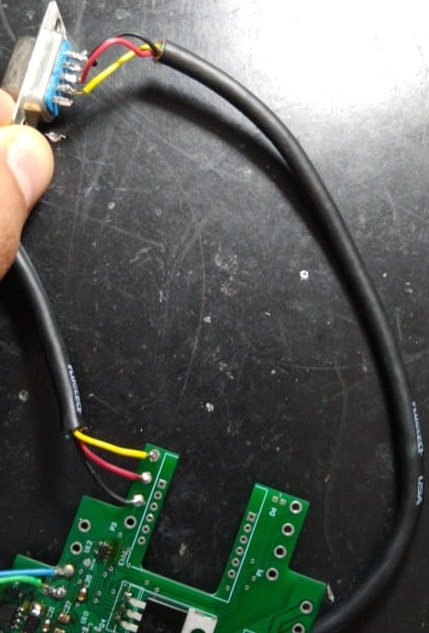
\includegraphics[width=80mm ,keepaspectratio]{Figures/ConRS232.jpeg}
	\caption{ Prueba de la interfaz RS232.}
	\label{fig:Rs232prott}
\end{figure}
La interfaz RS485 fue conectada exitosamente a través de un adaptador de nivel por puerto serie a la computadora, y utilizada durante las pruebas de protocolo Modbus.

Se instaló en el prototipo el módulo wiz820io, de puerto Ethernet, para que en el futuro se pueda programar en el dispositivo una interfaz Ethernet.

%Se establecieron dos salidas diferentes de la placa por las cuales cada una funciona por un estándar diferente. Se adaptaron los niveles de tension para que cada salida fuera capaz de manejar los protocolos deseados.

%\begin{itemize}
%\item Deberá contemplar una posible modificación a futuro para una interfaz ethernet a través de una entrada para rj45.
%\end{itemize}

%Se dejo en el PCB el grabado del footprint de un modulo wiz820io con puerto ethernet y se realizaron los cortes necesarios para que quepa en la carcasa para riel DIN.
 

\subsection{Grupo de requerimientos referidos a diseño del circuito eléctrico}
%\begin{itemize}
%\item El dispositivo deberá poseer como microcontrolador principal MSP430F2418
%\end{itemize}

%Se uso el microcontrolador MSP430F2418 de \textit{texas instrument} con una %referencia de tensión externa y un cristal oscilador de 32768 Hz.

%\begin{itemize}
%\item Se implementaran protecciones contra sobretensión en salida y entradas
%\end{itemize}

%La entrada de alimentación, y la salida de enlace de corriente tienen %protección de sobretensión. 

%\begin{itemize}
%\item Deberá poseer un relé para realizar un corte por corriente.
%\end{itemize}

%Se conecto al microcontrolador un relé para accionarlo según las necesidades.

Se usó el microcontrolador MSP430F2418 de Texas Instruments con una referencia de tensión externa y un cristal oscilador de 32768 Hz. Este puede verse soldado en la placa en la figura \ref{fig:polyrele}.

%\begin{figure}[!htb]
%	\centering
%	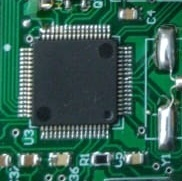
\includegraphics[width=80mm,keepaspectratio]{Figures/miccroenplaca.jpeg}
%	\caption{Microcontrolador soldado.}
%	\label{fig:microenplaca}
%\end{figure}

Un polyswitch que protege a la placa de sobre corriente puede verse en la figura \ref{fig:polyrele} en el sector superior derecha, también puede verse en la misma figura, en la parte inferior derecha, un relé soldado.

\begin{figure}[!htb]
	\centering
	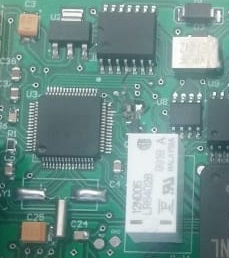
\includegraphics[width=80mm,keepaspectratio]{Figures/polyswitchyrele.jpg}
	\caption{ Area del microcontrolador en el dispositivo.}
	\label{fig:polyrele}
\end{figure}

\subsection{Grupo de requerimientos referidos a diseño  de impresión del circuito}

El diseño de la parte inferior del PCB se realizó teniendo en cuenta que el tipo de soldado fuese por ola de refusión. Los componentes fueron alineados teniendo en cuenta si provocarían sombras de estaño. El diseño puede verse en la figura \ref{fig:PCBbackk}.

%\ref{fig:PCBfrontt}.




 
%\begin{itemize}
%\item Se contempla en el diseño que el tipo de soldado será por refusión por cara superior.

%\item Se contempla en el diseño que el tipo de soldado será por ola en la cara inferior del circuito.
%\end{itemize}

%Ambos requerimientos se cumplieron en la elaboración del prototipo.

%\section{Realización de un manual de usuario}

%Al finalizar las correcciones sobre el software se elaboro un manual de %usuario en un documento online publico donde se especifica el uso del %dispositivo armado, sus partes y conexiones, especificaciones de que %parámetros puede medir y los registros que comunica por protocolo modbus.


%\begin{figure}[!htb]
%	\centering
%	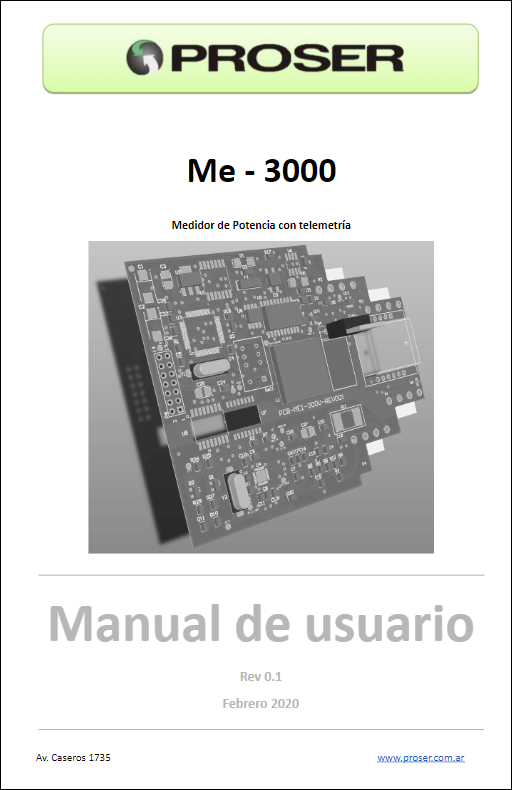
\includegraphics[width=80mm,keepaspectratio]{Figures/portadamanual.png}
%	\caption{Portada del manual elaborado.}
%	\label{fig:ManualPortad}
%\end{figure}

